\chapter{Regresión}
La palabra \emph{regresión} fue introducida por Francis Galton (1822-1911), haciendo referencia a que los hijos de personas altas, tendían a ser más bajos que sus padres,  fenómeno que denominó \textbf{Regresión a la media}. Este mismo fenómeno se puede observar cuando la segunda película de una saga no es tan buena como la primera parte. \\
La regresión es un método para estudiar la relación entre una variable $Y$, y otra variable independiente $X$, denominada característica. 
\begin{definition}[Función de Regresión] Se define la función de regresión $r(x)$ como:
$$
r(x)=\mathbb{E}(Y|X=x)=\int yf(y|x)dx
$$

\end{definition}
La idea de este método consiste en, dados datos $\mathcal{D}=\left \{ x_i,y_i \right \}_{i=1}^{n}$, encontrar una distribución $F_{X,Y}$. 
\section{Regresión Lineal Simple}
Comencemos viendo el caso unidimensional, es decir $X_i \in \R$. Buscamos ajustar $r(x)$ de forma tal que: 
$$
r(x)=\beta_0 + \beta_1 x,
$$

 es decir, de forma que y sea una función lineal (o lineal a fin ) de x. 
Supondremos que hay un ruido $\varepsilon_i$ tal que $\mathbb{V}(\varepsilon_i)=\sigma^2$, y es independiente de $x$. \\
\begin{definition}
Se define el modelo de regresión lineal simple como: 
$$
Y_i=\beta_0+\beta_1 X_i+ \varepsilon_i,
$$
con $\mathbb{E}(\varepsilon_i)=0$, y $\mathbb{V}(\varepsilon_i)=\sigma^2$.
\end{definition}
Buscamos estimar $\beta_0$ y $\beta_1$ de forma que tengamos una aproximación lineal que sea lo mejor posible. Estas últimas palabras nos hacen preguntarnos ¿Los mejores estimadores con respecto a qué? La respuesta es, con respecto a la métrica de mínimo cuadrados: 
$$
J(\hat{\beta_0},\hat{\beta_1})=\dfrac{1}{2} \sum_{i=1}^{n}(Y_i-\hat{Y_i})^{2},
$$
donde $\hat{Y_i}=\hat{\beta_0}+\hat{\beta_1}X_i$. 
\begin{theorem}
Los estimadores de mínimos cuadrados son: 
$$
\hat{\beta_1}=\dfrac{\sum_{i=1}^{n}(X_i-\bar{X})(Y_i-\bar{Y_i})}{\sum_{i=1}^{n}(X_i-\bar{X})^{2}}
$$
$$
\hat{\beta_0}=\bar{Y}-\hat{\beta_1}\bar{X}
$$
Un estimador insesgado de $\sigma^2$ es:
$$
\hat{\sigma^2}=\dfrac{1}{n-2} J(\hat{\beta_0},\hat{\beta_1})
$$
\end{theorem}
\section{Mínimos Cuadrados y Máxima Verosimilitud}
Supongamos ahora que $\varepsilon \sim \mathcal{N}(0,\sigma^2$, es decir, 
$Y_i|X_i \sim \mathcal{N}(\mu_i,\sigma^2)$, con $\mu_i=\beta_0 + \beta_1 X_i$.
Calculemos la verosimilitud: 
$$
\mathcal{L}=\prod_{i=1}^{n}f_{X}(X_i) f_{Y|X}(Y_i|X_i)= \prod_{i=1}^{n}f_{X}(X_i) \prod_{i=1}^{n}f_{Y|X}(Y_i|X_i)
$$
Llamemos $\mathcal{L}_1$ a la primera parte de este producto, y $\mathcal{L}_2$ a la segunda parte. Como $\mathcal{L}_1$ no depende de $\beta_0 $ y $\beta_1$, tenemos que para calcular los estimadores de máxima verosimilitud de estos parámetros, nos importa el segundo parámetro. Entonces, considerando la log-verosimilitud de $\mathcal{L}_2$:

$$ \mathcal{L}_2 = \prod_{i=1}^{n} f_{Y|X}(Y_i|X_i) \propto \sigma^{-n} exp(\dfrac{-1}{2\sigma^2}\sum_{i} (Y_i-\mu_i)^2) 
$$ 
$$
\implies l=-nlog(\sigma)-\dfrac{-1}{2\sigma^2}\sum_{i=1}^{n}(Y_i-(\beta_0 + \beta_1 X_i)^2
$$
Notemos que al minimizar esto, como el primer término es constante con respecto a $\beta_0 $ y $\beta_1$, tenemos: 
\begin{theorem}
Bajo la hipótesis de normalidad, el estimador de mínimos cuadrados coincide con el estimador de máxima verosimilitud. También se tiene: 
$$
\hat{\sigma}^2=\dfrac{1}{n} \sum_{i=1}^{n}(Y_i-\hat{Y_i})
$$
\end{theorem}
\begin{remark}
El estimador anterior de $\hat{\sigma}^2$ normalmente se reemplaza por el estimador insesgado de la parte anterior. 
\end{remark}

Lo anterior se puede extender al caso en que $X \in R^{k}$ de la siguiente forma. Suponemos: 
$$
Y_i= \sum_{j=1}^{k}\beta_j X_ij + \varepsilon_i,
$$
con $\mathbb{E}(\varepsilon_i)=0$. Denotemos:
$$
Y=\begin{pmatrix}
Y_1 \\
Y_2\\
.\\
.\\
.\\
Y_n\\
\end{pmatrix} ; 
X= \begin{pmatrix}
X_1 \\
X_2\\
.\\
.\\
.\\
X_n\\
\end{pmatrix}
$$
Cada fila de la matrix en $\R^{n \times k }$ $X$ es una observación. Sean:
$$
\beta= \begin{pmatrix}
\beta_1 \\
\beta_2\\
.\\
.\\
.\\
\beta_n\\
\end{pmatrix} \text{ y }
\varepsilon= \begin{pmatrix}
\varepsilon_1 \\
\varepsilon_2\\
.\\
.\\
.\\
\varepsilon_n\\
\end{pmatrix}
$$
Entonces: 
$$
Y=X\beta + \varepsilon
$$
\begin{theorem}
Si la matriz $X^{T}X$ es invertible: 
$$
\hat{\beta}= (X^{T}X)^{-1}X^{T}Y
$$
$$
\mathbb{V}(\hat{\beta})= \sigma^{2}(X^{T}X)^{-1}
$$
\end{theorem}

\begin{remark} Podemos tener observaciones de muchos $X_i$, pero no incluirlos todos al modelo. Un modelo más reducido tiene dos ventajas: La primera es que puede entregar mejores predicciones que un modelo más grande, y la segunda es que es más simple.\\  
Generalmente, mientras más variables se añaden a la regresión, el sesgo de la predicción disminuye pero aumenta la varianza. Una muestra pequeña genera mucho sesgo; esto se llama \emph{underfitting}. Una muestra muy grande lleva a una alta varianza; esto se llama \emph{overfitting}. Las buenas predicciones vienen de balancear sesgo y varianza. 
\end{remark}

\section{Regresión Logística}

\begin{definition}
Se llama función logística a la función: 
$$
f(x)=\dfrac{e^x}{1+e^x}
$$
\end{definition}
\begin{figure}[h]
    \centering
    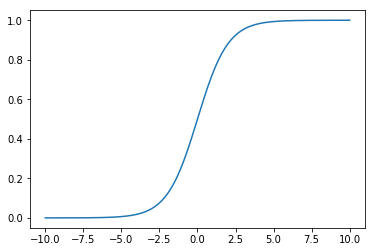
\includegraphics[scale=0.65]{img/funcion_logistica.png}
    \label{fig:logistica}
    \caption{Función Logística}
\end{figure}
La regresión logística es un método de regresión para el caso en que $Y_i \in \left \{0,1 \right \}$. El modelo considera: 

$$
p_i \equiv p_i(\beta) \equiv \mathbb{P}(Y_i=1 | X=x)= f(\beta_0+\sum_{j=1}^{k}\beta_{j} x_{ij}),
$$ 

con $f$ la función logística. De forma equivalente, si definimos $logit(p)=log(\dfrac{p}{1-p})$: 

$$
p_i=logit(p_i)= \beta_0+\sum_{j=1}^{k}\beta_j x_{ij}
$$

Como $Y_i$ son variables binarias, se tiene que   $Y_i|X_i=x_i \sim Ber(p_i)$. Así, la función de verosimilitud será:
$$
\mathcal{L}=\prod_{i=1}^{n} p_i(\beta)^{Y_i}(1-p_i(\beta))^{1-Y_i}
$$
Obtenemos el estimador de $\beta$, $\hat{\beta}$ usando método numéricos de optimización. 